\documentclass[12pt,titlepage]{article}
\usepackage{graphicx}
\author{The TOME Team}
\title{\textbf{TOME Project Brief}}
\begin{document}
\maketitle
\tableofcontents
\listoffigures
\newpage
\section{Introduction}
\subsection{Purpose}
The purpose of this Project Brief is to document the \textbf{initial} ideas for TOME.

It is emphasized that all sections of this document will be refined and expanded upon in the Business Investigation Phase.  It is not the purpose of this document to provide detailed costs, benefits and schedules as these will be developed in later Phases.

\subsection{Scope}
This document:
\begin{itemize}
	\item Identifies details of the project
	\item States the purpose and objectives of the project
	\item States the scope of the project
	\item Identifies the risks associated with the project
\end{itemize}
\subsection{Audience}
This document is directed to all personnel who may be considered stakeholders in the initiation, development, implementation, and ongoing support for this project.
\section{Project Details}
\textbf{Title:} TOME\\
\textbf{Initiation Date:} September 5, 2006\\
\textbf{Sponsoring Organization:} LeTourneau University Computer Science Department\\
\textbf{Team Lead:} Curtis ``Fjord'' Hawthorne
\section{Project Overview}
\subsection{Problem Definition}
Currently, when students are finished with a book they are using for the semester, they only have a few choices: keep the book, sell it to the bookstore or on the internet, or let a friend borrow it.  Keeping the book does not make any sense if the student is not likely to read it again, and selling the book usually results in a significant loss of money.  Letting a friend borrow the book is a great use of the book, but it can be difficult for the book owner to find out who needs what books and for the prospective borrower to determine what books are available for borrowing.
\subsection{Purpose of Project}
TOME is a solution to the problem of book borrowing.  Instead of the disorganized and inefficient borrowing that occurs naturally, TOME is an organized, centralized system.  All books for a region (such as a campus floor) are donated to a central repository and entered into a database.  This repository is generally a closet or bookshelf in the TOMEkeeper's room.  This database keeps track of not only which books are available and which have been checked out, but also what books go with what classes.  Currently, books are checked out on a first come, first serve basis, and all checkouts are done free of charge.  Because the system is run by TOMEkeepers and not users, needs can be worked around as they arise.  Books are donated to the library for free.  Types of book are managed by ISBN.  This works well because every edition of every book has a unique ISBN.  TOME should make the book acquisition process as painless as possible for as many students as possible.
\subsection{Current Situation}
TOME is already quite robust and successful.  It consists of a web front end that the TOMEkeepers use to manipulate a PostgreSQL database.  The database has many built-in consistency checks.  The underlying program is made with Apache, Perl, and a number of Perl modules.  The details of this can be seen in the Trac Wiki.
\begin{figure}[h]
	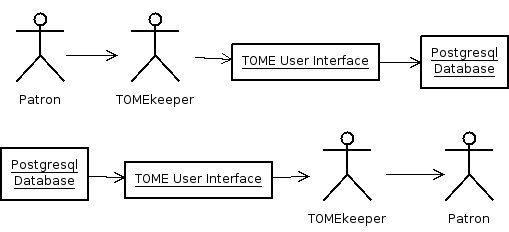
\includegraphics[width=\textwidth]{userdiagram}
	\caption{TOME Actor Diagram}
\end{figure}
\subsection{References}
All project data will be stored in a combination Subversion repository and Trac environment.  All of this will be made viewable at the following URL:

\texttt{http://enosh.letnet.net/trac/tome}
\subsection{Project Goals}
\begin{description}
	\item[Automated Test Suite] This suite will be capable of creating a blank TOME database, starting a self-contained webserver, using the system like a normal user would, and checking the web and database output of the system.
	\item[Patron-Centric Work Flow] TOME will be reorganized to focus the entire work flow of selecting classes, reserving books, and making checkouts to be centered around patrons instead of books.  This will make the job of the TOMEkeeper much easier.
	\item[ISBN-Based Reservations] All reservations will be made on an ISBN basis instead of for specific book IDs.  Instead of reserving a specific, physical instance of a book, reservations will be made for ISBNs, and the database will ensure that the number of books reserved by ISBN does not exceed the number of physical books available.
	\item[InterTOME Loans] The InterTOME Loan System will be reworked following research with TOMEkeepers and an analysis of the shortcomings of the current system.
	\item[Documentation] The installation process for the system will be thoroughly documented, and current administrative documentation will be expanded.
	\item[Usability] The look and feel of TOME will be improved.
\end{description}
\section{Operational Vision}
Each team member is expected to contribute approximately six hours of work every week.  In addition, every team member should attend weekly team meetings where past progress and future direction will be discussed.  Project responsibilities will be roughly broken down as follows:
\begin{description}
	\item[Curtis ``Fjord'' Hawthorne] Team Lead.  Responsible for core design changes and implementation.
	\item[fREW Schmidt] Responsible for intermediate-level design and implementation.
	\item[Craig ``Fargo'' Miller] Responsible for presentation-level design and implementation.
	\item[Clint Olson] Responsible for test suite design and implementation.
\end{description}
These roles are not set in stone, and some degree of overlap is expected to happen.  However, these will function as general guidelines for the duration of the project.
\section{Risk Assessment}
The project contains risks that will require monitoring to ensure that they are minimized and do prevent a successful, on time delivery.

These risks are identified below:
\begin{description}
	\item[Project left in an unusable state] All development will be kept in Subversion.  At the very least, the project can be rolled back to its current, working condition.  However, as a policy, no changes will be committed until the system is in a usable state.
	\item[New work flows are not an improvement] No changes will be made to the work flow of the system without first discussing the changes with experienced users of the system.
	\item[Maintainability concerns] The project's installation procedure, code, test suite, and overall structure will be documented.
\end{description}
\end{document}
